\section{Technical Specification} \label{sec:Technical}

Generally all SCM platform has three main items: Assets (the product or goods itself), steps (phases which products go through) and actors (people who interact with the products during the steps). The platform is based on this triad and it must be well defined on a new supply chain's creation. Initially, a configuration file in json format is generated and read in the blockchain platform, adding the main information for the correct functioning of the chain. The mechanism for creating this configuration file is detailed in the sections \Cref{sec:UserInteraction,sec:ServiceLayer} {\color{red} VERIFICAR AQUI SE A SUBSEÇÃO ESTÁ CORRETA}.

The general objective of this work is to create a generic framework intended to be used in any kind of supply chain correlated to assets and products. Árion project is divided into three main modules described below: WebApp - FrondEnd, WebApp - BackEnd and Data Storage. Figure~\ref{fig:detalhamentotecnico} shows the application architecture and its components.

%htbp
\begin{figure}[ht]
\begin{center}
  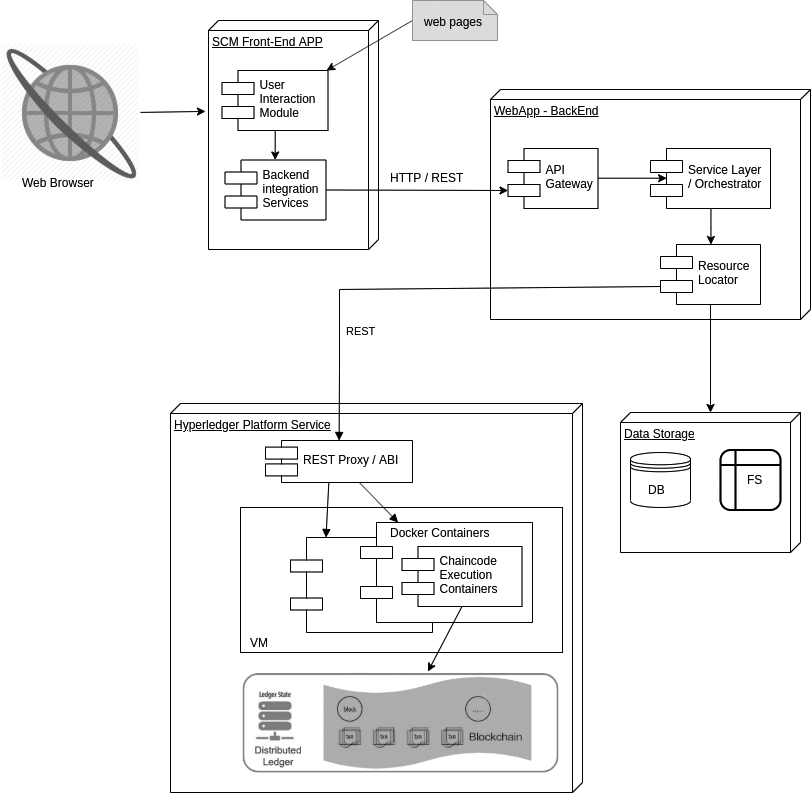
\includegraphics[scale=0.45]{images/detalhamentotecnico.png}
\caption{Árion Application architecture}
\label{fig:detalhamentotecnico}
\end{center}
\end{figure}

\subsubsubsection{Chaincode}
{\color{red} ??? adicionar aqui as informações do codigo golang criado}

\subsection{WebApp - FrondEnd}\label{sec:WebAppFrondEnd}
WebApp - FrontEnd is a client–server application which the client (including the user interface and client-side logic) runs in a web browser. This is a single-page application (SPA) that interacts with the user by dynamically rewriting the current page rather than loading entire new pages from a server. This approach avoids interruption of the user experience between successive pages, making the application behave more like a desktop application.

The application is build with React (also known as React.js or ReactJS). This is a JavaScript library for building user interfaces. Used as a base in the development of single-page or mobile applications, React is optimal for fetching rapidly changing data that needs to be recorded. However, fetching data is only the beginning of what happens on a web page, which is why complex React applications usually require the use of additional libraries for state management, routing, and interaction with an API. The Webapp - FrontEnd is divided into two main blocks and these are classified according to the interactions: User Interaction Modules and Backend Interactions Services.

\subsubsection{User Interaction}\label{sec:UserInteraction}
The User Interaction modules are responsible for providing web pages that will be rendered on client’s web browser. These interactions are provided by web pages grouped by the following modules:

\begin{itemize}
\item Login page
\item Application configuration module
\item User handling module (actors - CRUD)
\item Data entry module (forms)
\item Data visualization module
\item Reporting module
\end{itemize}

The Login Module is responsible for display the login and authentication alternatives pages (‘forgot my password’, ‘reset my password’, etc.). The Application configuration module provides the features of creation/configuration of supply chain items and supply chain flows (steps). This module is responsible for get the information from the user that will be used for generate the configuration json file in the backend. This module provides the features for creation/configuration of Actors and Roles. These info will complement the main configuration file. The Data entry module provides form pages that allow the actors to enter data in the application, search and move assets from a step to another. The Data visualization module is responsible to display the information about assets in the supply chain flow through steps. In the Reporting module users can generate reports/files containing information organized in a narrative, graphic, or tabular form, prepared on ad hoc, periodic, recurring, regular, or as required basis. Reports may refer to specific periods, events, occurrences, or subjects, and may be presented in written form or any other format.

\subsubsection{Backend Interaction}\label{sec:BackendInteraction}
Backend interactions happen via a service layer consisting of:

\begin{itemize}
\item Authentication service
\item Application setup service
\item User creation service
\item Data entry service
\item Data visualization service
\item Reporting service
\end{itemize}

The function of the Authentication Service is to request information from an authenticating party, and validate it against the configured identity repository using the specified authentication module. After successful authentication, the user session is activated and can be validated across all web applications participating in an Single Sign-On (SSO) environment. For example, when a user or application attempts to access a protected resource, credentials are requested by one (or more) authentication modules. Gaining access to the resource requires that the user or application be allowed based on the submitted credentials.

Application setup service provides methods to configure and edit  supply chain items and supply chain flows, defining which steps and sub-tasks will be present in this flow and which information will be present in these steps. The User creation Service is responsible for the creation of users and roles, to allow them to log in and use the application’s features. Data entry service receives data from UI forms and send them to the backend to be processed and stored. Data visualization services provides information about the supply chain: Assets, actors and transactions, to be used by the data visualization module. Report services generate files (Doc/PDF/XSL, etc...) from a specific period of time with information about the supply chain.

\subsection{WebApp - BackEnd}\label{sec:WebAppBackEnd}
WebApp - BackEnd is a Middleware that runs on the server. This Middleware (server-side software) facilitates client-server connectivity, forming a middle layer between the app(s) and the network: the server, the database, the operating system, and more. It receives requests from the clients (in this case, the WebApp - FrontEnd), and contains the logic to send the appropriate data back to the applicant, over HTTP and REST.  These are the main conventions that provide structure to the request-response cycle between clients and servers. Built with Node.js, This module  is composed by the API Gateway, Service Layer and Resource Locator more detailed below.

\subsubsection{API Gateway}\label{sec:APIGateway}
API Gateway is a managed service that enables easily create, publish, maintain, monitor and secure REST APIs to act as a "gateway" for applications to access data, business logic, or functionality in the backend services, such as workloads. The API Gateway provides a simple uniform view of external resources to the internals of an application. It manages all tasks involved in receiving and processing API calls, including traffic management, authorization and access control, monitoring and management of API versions.

Basically, the Gateway is an interface that receives calls to its internal systems and can act in five different ways:

\begin{itemize}
\item Filter for call traffic from different media (web, mobile, cloud, among others);
\item Single gateway to the various APIs you want to expose;
\item Essential component of API management, as API Suite;
\item Router: API and Rate Limit traffic router;
\item Security engine with authentication, logging and more.
\end{itemize}

Gateway access can be done from many different devices. Therefore, it must have the power to unify outgoing calls and be able to deliver to the user content that can be accessed from any browser and system. Gateways as a Security Feature: In the APIs world, one of the most subject talked about issues is always security, and having an API Gateway is one of the best solutions on the market to get full control of API’s, because this pattern addresses the so-called CIA (Confidentiality, Integrity, Availability) almost flawlessly.

\subsubsection{Service Layer}\label{sec:ServiceLayer}
A Service Layer defines an application's boundary [Cockburn PloP] and its set of available operations from the perspective of interfacing client layers. It encapsulates the application's business logic, controlling transactions and coordinating responses in the implementation of its operations.This module implements the service layer pattern and provides some benefits:

\begin{enumerate}
\item Centralizes external access to data and functions.
\item Hides (abstracts) internal implementation and changes.
\item Allows for versioning of the services.
\end{enumerate}

The service layer acts as an orchestrator, controlling the flow of incoming and outcoming information requests and responses. Orchestration allows to directly link process logic to service interaction within workflow logic. This combines business process modeling with service-oriented modeling and design, realizing workflow management through a process service model. Orchestration brings the business process into the service layer, positioning it as a master composition controller.

\subsubsection{Resource Locator}\label{sec:ResourceLocator}

Resource locators are components that abstracts the persistence layer. Their job is to provide an object that can help services to discover and persist information from/to the Data Storage Module. Information can be stored in the Blockchain, Filesystem or Database and resource locators should know exactly where get/put data within them.

\subsection{Data Storage}\label{sec:DataStorage}
Data storage is a general term for archiving data in electromagnetic or other forms for use by a computer or device. Different types of data storage play different roles in a computing environment. In addition to forms of hard data storage, there are now new options for remote data storage, such as cloud computing, and blockchain that can revolutionize the ways that users save and access data.  

Árion uses three applications as data storages: Blockchain, Cloud filesystem and relational database better detailed on next subsections. Blockchains grow continuously because of the amount of data and code in them, which is unchanging. Therefore, an important design decision is to choose which data and calculations to keep in and out of the chain.

\subsubsection{Blockchain}\label{sec:DataStorageBlockchain}
The platform uses Blockchain as a supply chain that track parts and service provenance, ensure authenticity of goods, block counterfeits and reduce conflicts.

To achieve that, Hyperledger Fabric is used. Hyperledger is an open source collaborative effort created to advance cross-industry blockchain technologies. It is a global collaboration, hosted by The Linux Foundation, including leaders in finance, banking, Internet of Things, supply chains, manufacturing and Technology.
Hyperledger Fabric is an enterprise-grade permissioned distributed ledger framework for developing solutions and applications. Its modular and versatile design satisfies a broad range of industry use cases. It offers a unique approach to consensus that enables performance at scale while preserving privacy.

In context of Árion, the Blockchain module consists in a smart contract, chaincode and the ledger. From the application developer’s perspective, a smart contract, together with the ledger, form the heart of a Hyperledger Fabric blockchain system. Whereas a ledger holds facts about the current and historical state of a set of business objects, a smart contract defines the executable logic that generates new facts that are added to the ledger. A chaincode is typically used by administrators to group related smart contracts for deployment, but can also be used for low level system programming of Fabric.

\subsubsubsection{Smart contract}
Before businesses can transact with each other, they must define a common set of contracts covering common terms, data, rules, concept definitions, and processes. Taken together, these contracts lay out the business model that govern all of the interactions between transacting parties.

A smart contract defines the rules between different organizations in executable code. Applications invoke a smart contract to generate transactions that are recorded on the ledger.

\subsubsubsection{Chaincode}
Hyperledger Fabric users often use the terms smart contract and chaincode interchangeably. In general, a smart contract defines the transaction logic that controls the lifecycle of a business object contained in the world state. It is then packaged into a chaincode which is then deployed to a blockchain network. Think of smart contracts as governing transactions, whereas chaincode governs how smart contracts are packaged for deployment.

\subsubsubsection{Ledger}
At the simplest level, a blockchain immutably records transactions which update states in a ledger. A smart contract programmatically accesses two distinct pieces of the ledger – a blockchain, which immutably records the history of all transactions, and a world state that holds a cache of the current value of these states, as it’s the current value of an object that is usually required.

Smart contracts primarily put, get and delete states in the world state, and can also query the immutable blockchain record of transactions.

\begin{itemize}
\item A \textbf{get} typically represents a query to retrieve information about the current state of a business object.
\item A \textbf{put} typically creates a new business object or modifies an existing one in the ledger world state.
\item A \textbf{delete} typically represents the removal of a business object from the current state of the ledger, but not its history.
\end{itemize}

Smart contracts have many APIs available to them. Critically, in all cases, whether transactions create, read, update or delete business objects in the world state, the blockchain contains an immutable record of these changes.

\subsubsection{Filesystem}\label{sec:Filesystem}
A cloud file system is a tiered storage system that provides shared access to file data. Users can create, delete, modify, read and write files, as well as logically organize them into directory trees for intuitive access.

Cloud file sharing can be defined as a service that gives multiple users simultaneous access to a cloud file data set. Cloud file sharing security is managed with user and group permissions, allowing administrators to tightly control access to shared file data.

For all file uploaded and stored in the filesystem, a locally stored digital fingerprint (hash) is saved in the blockchain, separately from the original files or content, to make it easier to confirm whether data has been altered or manipulated in a particular organization.

\subsubsection{Database}\label{sec:Database}
A relational database is a set of formally described tables from which data can be accessed or reassembled in many different ways without having to reorganize the database tables. The standard user and application programming interface (API) of a relational database is the Structured Query Language (SQL). SQL statements are used both for interactive queries for information from a relational database and for gathering data for reports.
